\documentclass[parskip=full]{scrartcl}
\usepackage[T1]{fontenc}    % avoid garbled Unicode text in pdf
\usepackage[utf8]{inputenc} % use utf8 file encoding for TeX sources
\usepackage[german]{babel}  % german hyphenation, quotes, etc
\usepackage{hyperref}       % detailed hyperlink/pdf configuration
\hypersetup{                % ‘texdoc hyperref‘ for options
pdftitle={PSE: Entwicklung eines relationalen Debuggers - Pflichtenheft},%
,%
}
\usepackage{graphicx}       % provides commands for including figures
\usepackage{csquotes}       % provides \enquote{} macro for "quotes"
\usepackage[nonumberlist]{glossaries}     % provides glossary commands
\usepackage{enumitem}

\makenoidxglossaries


\title{PSE:\\ Entwicklung eines relationalen Debuggers\\ Pflichtenheft}
\author{
	Benedikt Wagner\\
	\texttt{udpto@student.kit.edu}
	\and Chiara Staudenmaier\\
	\texttt{uzhtd@student.kit.edu}
	\and Etienne Brunner\\
	\texttt{urmlp@student.kit.edu}
	\and Joana Plewnia\\
	\texttt{uhfpm@student.kit.edu} 
	\and Pascal Zwick\\
	\texttt{uyqpk@student.kit.edu}
	\and Ulla Scheler\\
	\texttt{ujuhe@student.kit.edu}
}

\begin{document}

\maketitle
\newpage

\tableofcontents
\newpage

\section{Produktübersicht}
%kurze Übersicht über das Produkt
Das Produkt soll dem Nutzer die Möglichkeit bieten, mehr als ein Programm gleichzeitig zu debuggen und interaktiv zu analysieren. \\
Dabei sollen die Konzepte eines herkömmlichen Debuggers, namentlich Einzelschritte, Breakpoints und Variableninspektion, erhalten bleiben und um zusätzliche Konzepte, die den Umgang mit zwei oder mehr Programmläufen erleichtern, erweitert werden. Der Fokus liegt hierbei auf der Unterstützung des Findens von relationalen Zusammenhängen in den vom Nutzer in einer WHILE-Sprache, welche eine Teilmenge von Java darstellt und in Kapitel 12 näher definiert wird, verfassten Programmen.


\section{Produkteinsatz}
Das Produkt unterstützt das Institut für theoretische Informatik am Karlsruher Institut für Technologie beim Führen von Beweisen zu relationalen Eigenschaften von Programmen. Hierbei soll die Möglichkeit des gleichzeitigen Debuggens der Programme dem Nutzer bei der Beweisführung helfen. \\
Verwendet wird das Produkt hierbei von wissenschaftlichen Mitarbeitern am Lehrstuhl "Anwendungsorientierte formale Verifikation - Prof. Dr. Beckert" des Instituts für theoretische Informatik am Karlsruher Institut für Technologie und soll in deren Büroumgebung zum Einsatz kommen. 

%Anwendungsbereiche, Zielgruppen, Betriebsbedingungen
 

\section{Produktumgebung}
%Software, Hardware, Orgware, Schnittstellen
Das Produkt läuft auf dem Rechner des Nutzers und benötigt keine Kommunikation mit außerhalb. Hierbei läuft das Produkt eventuell neben anderen Applikationen, kommuniziert jedoch nicht mit diesen.

\subsection{Software}
Da es sich bei dem Produkt um ein Java-Programm handelt, muss ein JRE (Java Runtime Environment) auf dem Rechner vorhanden sein oder mitinstalliert werden. \\
Das Produkt läuft sowohl auf Windows, als auch auf Mac OS und Linux.

\subsection{Hardware}
An die Hardware des Rechners werden keine speziellen Anforderungen gestellt. Das Produkt läuft auf jedem Standardrechner (ca. 1 GHz und 128 MB RAM).

\subsection{Schnittstellen}
Das Produkt hat Schnittstellen zur graphischen Benutzeroberfläche und zum Interpreter, um diese leicht austauschbar zu gestalten. \\
Außerdem können durch eine öffentliche Schnittstellen, mittels austauschbarer Sprachkonfigurationsdateien, verschiedene Sprachen der Benutzeroberfläche genutzt werden. 


\section{Produktfuntionen}
	 	\subsection{Funktionale Anforderungen}
 		\subsubsection{Musskriterien}
		\begin{itemize}
		\item[/FA10/] Das Produkt ist ein Debugger für Quellcodes, welche in der im Kapitel Ergänzungen spezifizierten Sprache geschrieben sind.
		\item[/FA20/] Im Debugmodus kann der Benutzer Schritte(Steps) durchführen.
		\item[/FA30/] Es ist möglich unabhängige Einzelschritte in einem Programm auszuführen.
		\item[/FA40/] Der Benutzer kann die Schrittgröße für jedes Programm einzeln festlegen.
		\item[/FA50/] Bei einem Schritt wird die vorgegebene Anzahl an Befehlen ausgeführt. Dabei werden die Befehle einer Funktion einzeln ausgeführt (automatisches Step-In). 
		\item[/FA60/] Der Benutzer kann durch Step-Out eine Funktion verlassen.
		\item[/FA70/] Durch Step-Over kann eine Funktion als einzelner auszuführender Befehl abgearbeitet werden.
		\item[/FA80/] Der Benutzer kann Breakpoints an Zeilen im Code setzen.
		\item[/FA90/] Der Benutzer kann relationale Eigenschaften bezüglich Variablen als bedingte Breakpoints festlegen.
		\item[/FA100/] Bedingte Breakpoints können an vom Benutzer bestimmte Stellen im Code gebunden werden.
		\item[/FA110/] Der Benutzer kann relationale Eigenschaften bezüglich Variablen als Watch-Expressions festlegen.
		\item[/FA120/] Watch-Expressions können an vom Benutzer bestimmte Stellen im Code gebunden werden.
		\item[/FA130/] Im Debugmodus kann der Benutzer durch Auswahl der Option Weiter das Programm bis zum nächsten Breakpoint debuggen.
		\item[/FA140/] Das Produkt bietet die Möglichkeit, eine Konfigurationsdatei für einen Lauf zu speichern. Diese beinhaltet festgelegte Eingabewerte, Breakpoints, Watch-Expressions, Schrittgröße und die zu debuggenden Codes.
		\item[/FA150/] Das zu debuggende Programm kann direkt in die Textbox des Produkts  geschrieben werden.
		\item[/FA160/] Das zu debuggende Programm kann direkt in die Textbox des Produkts kopiert werden.
		\item[/FA170/] Das zu debuggende Programm kann aus einer Textdatei eingebunden werden.
		\item[/FA180/] Der Debugmodus kann vom Benutzer abgebrochen werden. Dadurch kehrt der Benutzer zum Editiermodus zurück.
		\item[/FA190/] Nach jedem Schritt oder Breakpoint werden die aktuellen Variablenbelegungen angezeigt.
		\item[/FA200/] Die Variablenreihenfolge im Variableninspektor ist manuell veränderbar.
		\item[/FA210/] Im Variableninspektor können Variablen ausgeblendet werden.
		\end{itemize}
 
 		\subsubsection{Sollkriterien}
		\begin{itemize}
		\item[/FA220/] Das Produkt kann zufällige Vorschläge für Eingabewerte über einen Vorschlag-Button erstellen. Der Benutzer kann diese noch ändern.
		\item[/FA230/] Der Benutzer kann Variablen auswählen, von welchen jeder angenommene Wert gespeichert wird.
		\item[/FA240/] Bei Endlosschleifen wird automatisch abgebrochen. Die maximale Anzahl an Schleifendurchläufe kann vom Benutzer festgelegt werden (maximal 250).
		\item[/FA250/] Der Benutzer kann mehr als zwei Programme simultan debuggen.
		\end{itemize}

 		\subsubsection{Kannkriterien}
 		..
 		\subsubsection{Abgrenzungskriterien}
	\subsection{Nichtfunktionale Anforderungen}
		\subsubsection{Produktdaten}
			\paragraph{/PD10/ Konfigurationsdateien:}
			Diese Dateien speichern eine Konfiguration des Debuggers.
			Zu diesen gehören die Eingabewerte, Schrittgrößen, Variablen Auswahl, 						Quelltext und Position beider Programme, aber nicht die Ausgabewerte, da diese 			vom Programmcode zur Laufzeit generiert werden.
			Weiter müssen alle Breakpoints gespeichert werden. Dazu zählen sowohl gesetzte 			als auch bedingte Breakpoints. Letzteres benötigt keine Speicherung der Zeile, 			sondern eines Bereiches, zweier Variablen der Programmtexte und eines Operators. 				Dies gilt auch für die Watch-Expressions mit Ausnahme eines Bereiches.
			\paragraph{/PD20/ Sprachdateien:}
			Diese Datei speichert die Übersetzung der gesamten Benutzeroberfläche.
			Dazu gehören die Texte auf GUI-Elementen und Tooltips.
			\paragraph{/PD30/ Einstellungsdatei:}
			Diese Datei speichert die zuletzt ausgewählte Sprache und die URL der 						Konfigurationsdatei, welche zur zuletzt verwendeten Konfiguration passt.
		\subsubsection{Produktleistungen}
		..
		\subsubsection{Weitere nichtfunktionale Anforderungen}
		..

\section{Qualitätsanforderungen}
..

\newpage
\section{Anwendungsfälle und Szenarien}
\begin{figure}[h] 
  \centering
     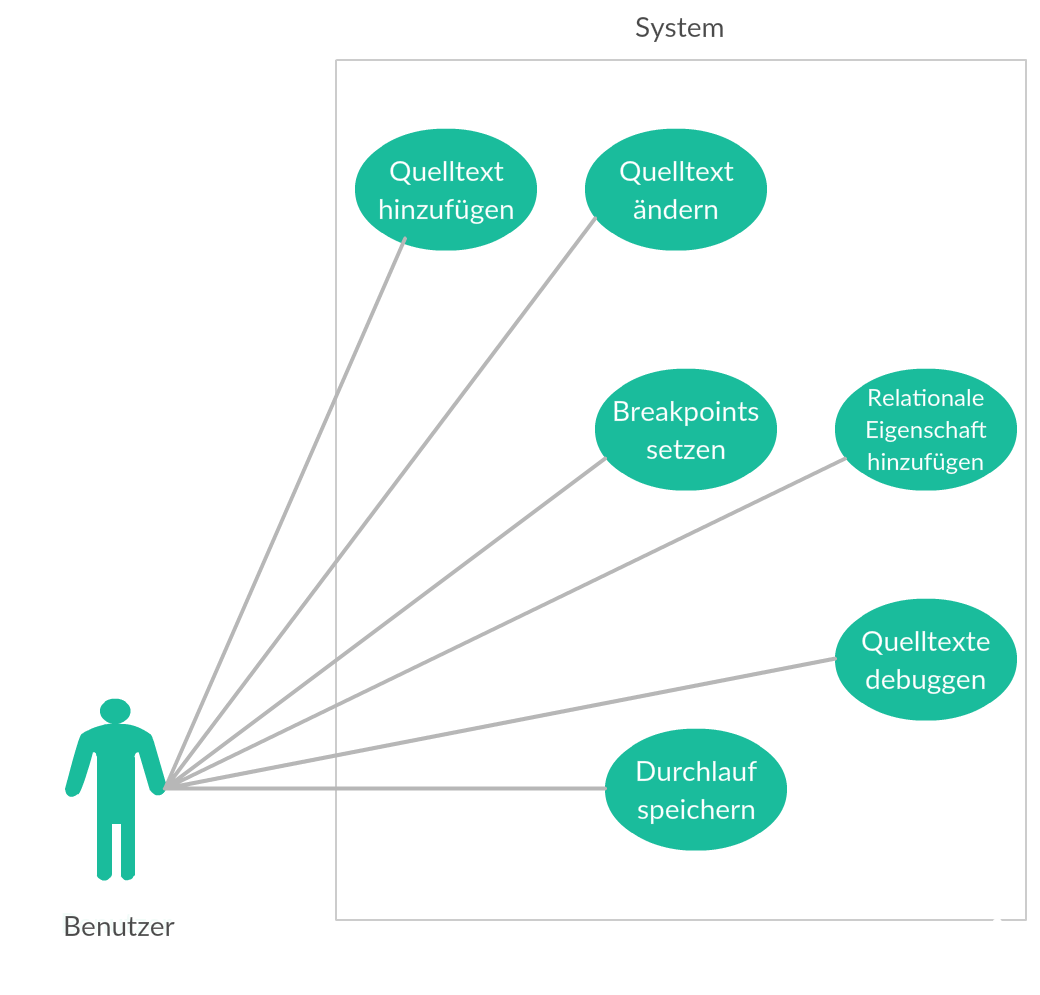
\includegraphics[width=0.7\textwidth]{Anwendungsfalldiagramm}
  \caption{Anwendungsfalldiagramm}
  \label{fig:Bild1}
\end{figure}

\section{Globale Testfälle}
..

\newpage
\section{Systemmodelle}
%Architektur, Verhalten, usw
\begin{figure}[h] 
  \centering
     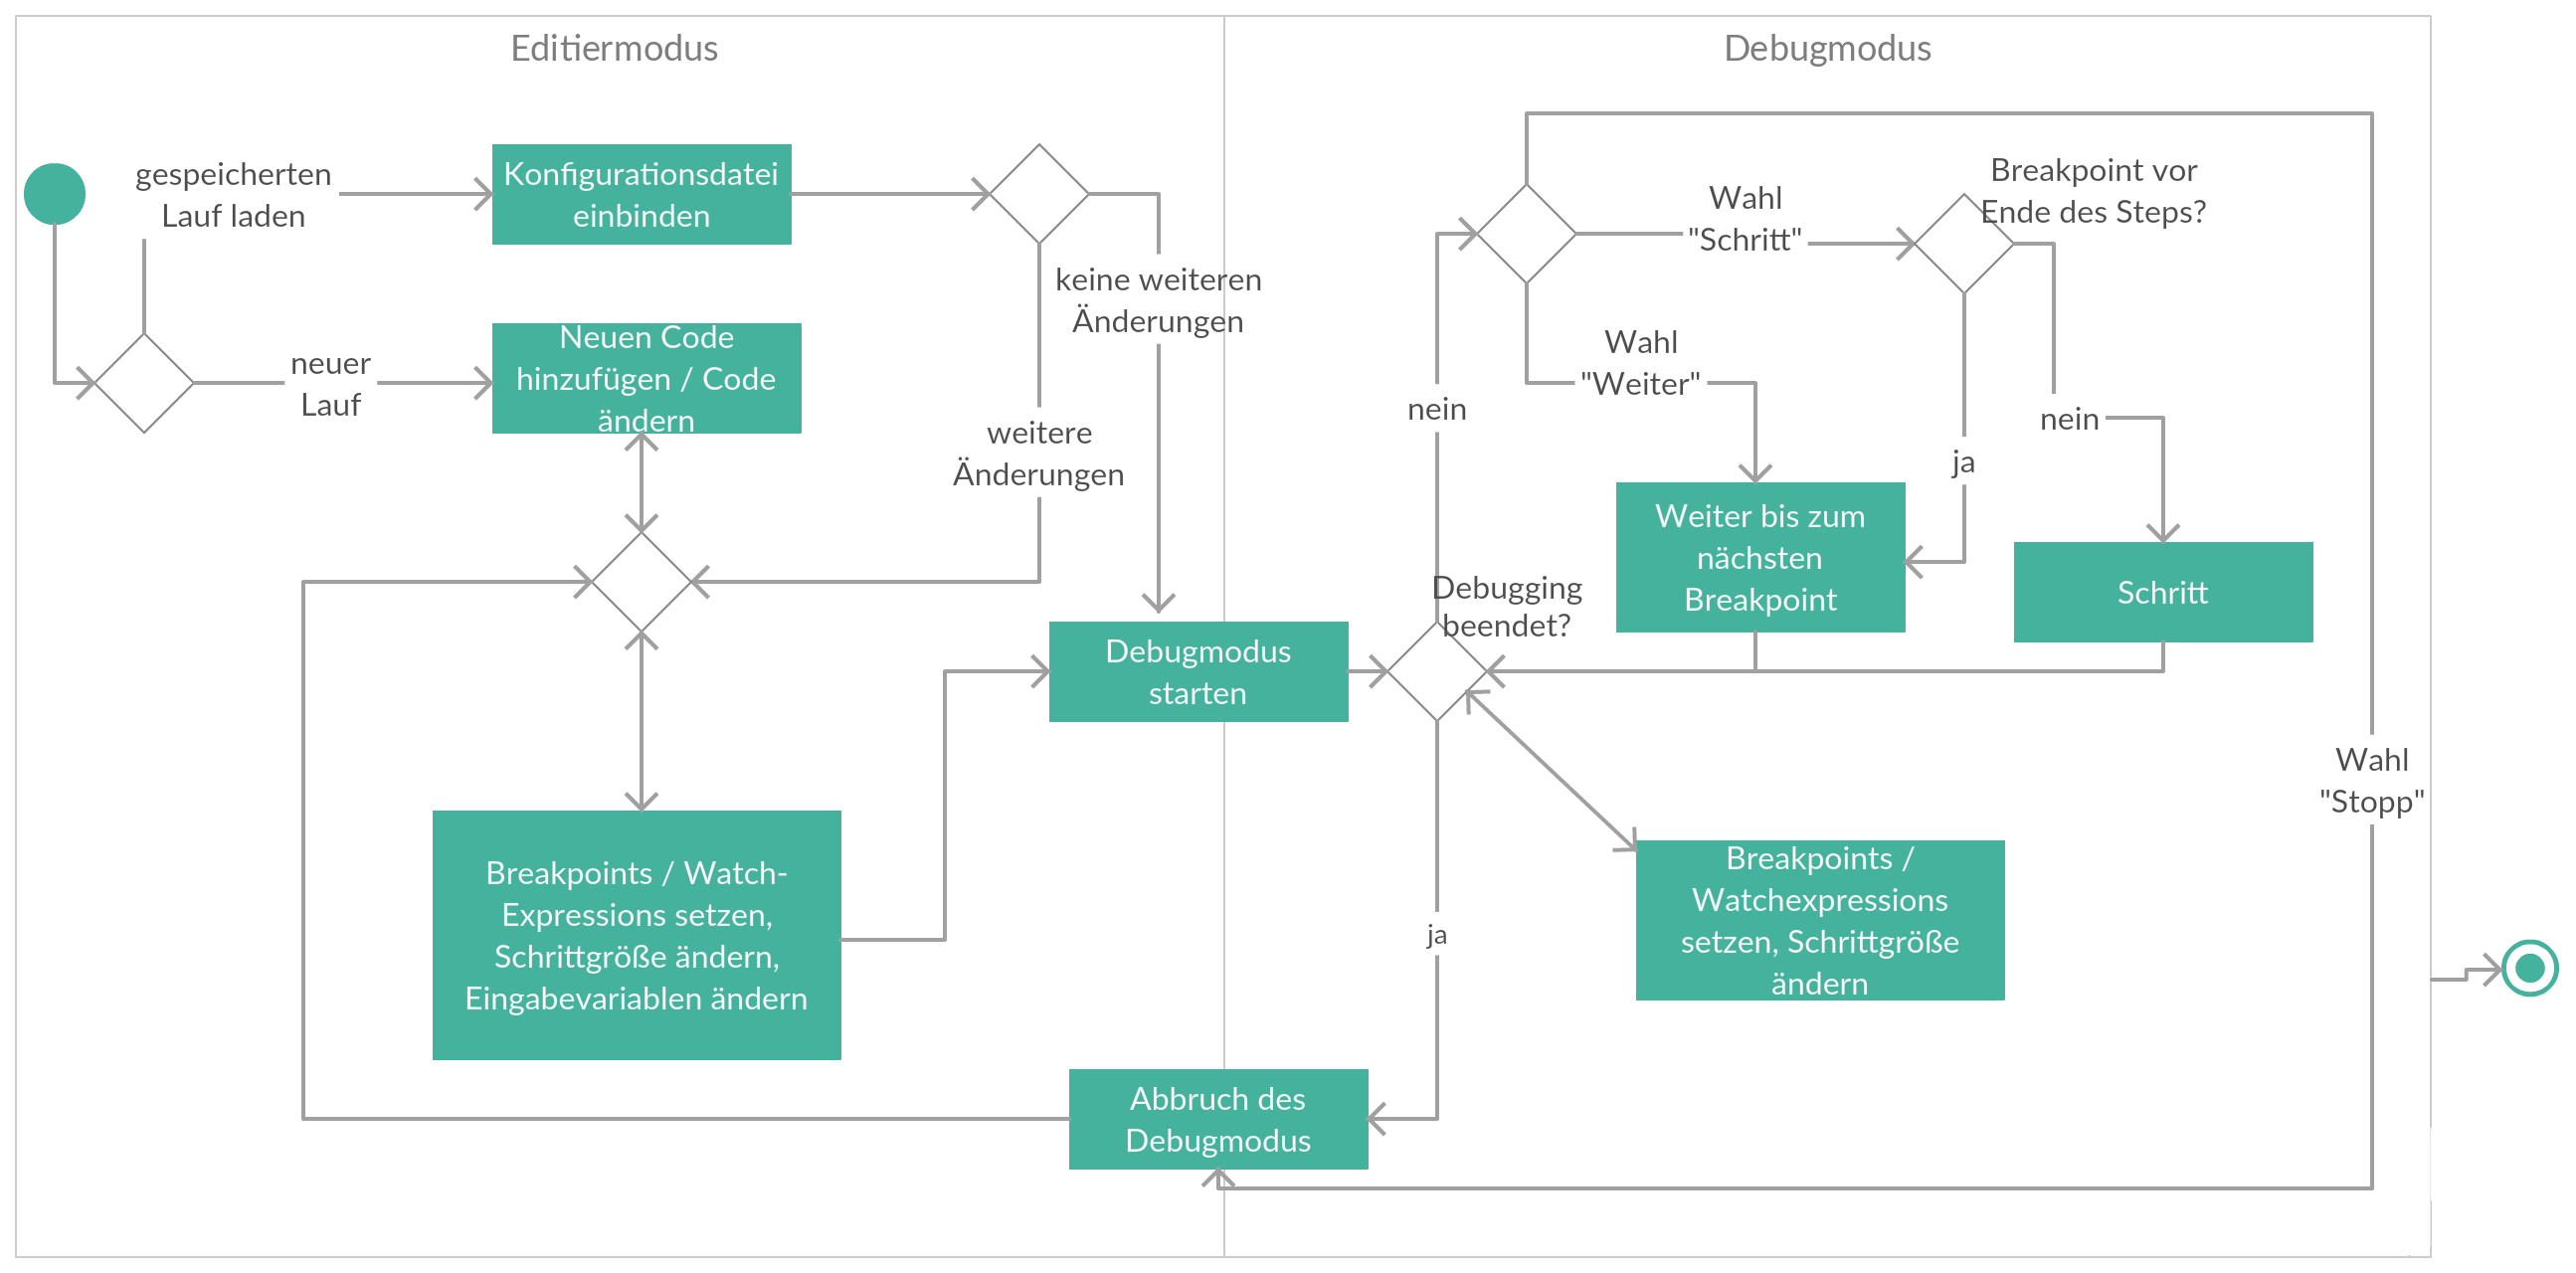
\includegraphics[width=0.9\textwidth]{Aktivitaetsdiagramm}
  \caption{Aktivitätsdiagramm}
  \label{fig:Bild1}
\end{figure}

\newpage
\section{Benutzungsoberfläche}
%Gui-Skizzen, Erklärungen der Menüs, usw
\begin{figure}[!ht] 
    \vspace{-10pt}
    \centering
       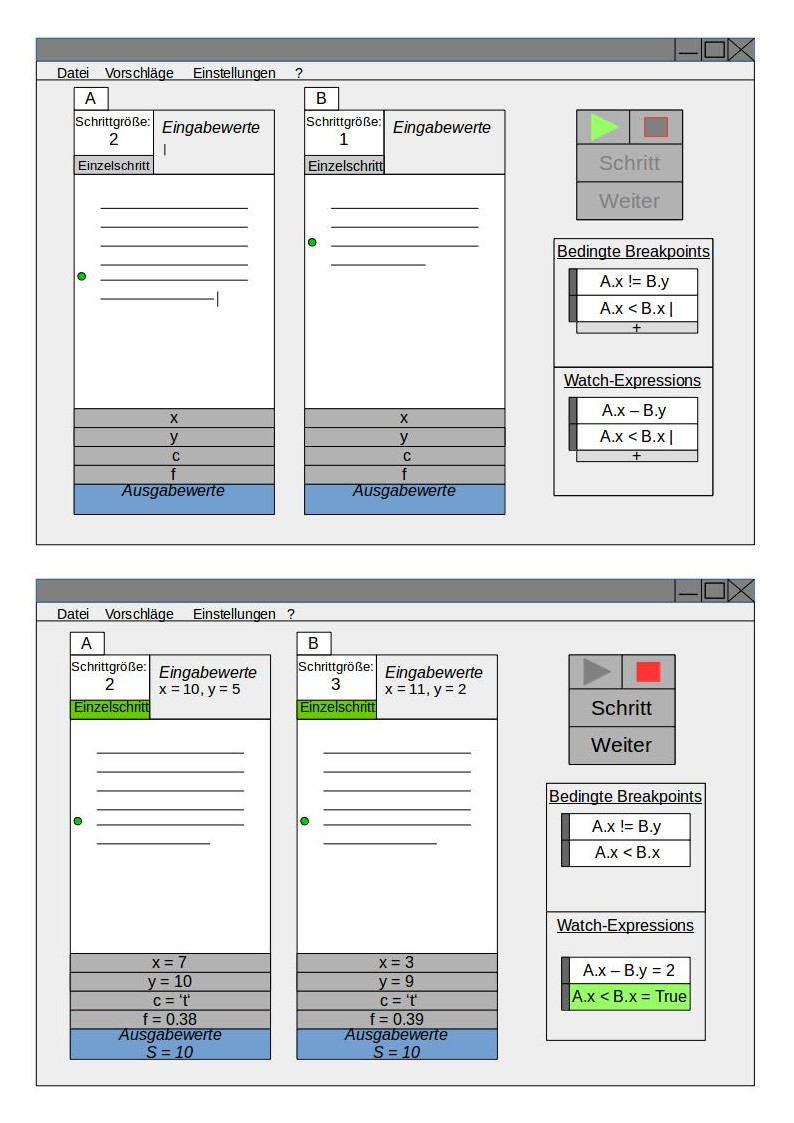
\includegraphics[width=0.7\textwidth]{skizzeFull.jpg}
       \caption{
         Benutzeroberfläche von --Programmname-- im Editiermodus (oben) und im Debugmodus
         (unten)
       }
    \label{fig:Bild1}
\end{figure}

    \subsection{Beschreibung}
        Befindet sich --Programmname-- im Editiermodus, so können die Eingabequelltexte über die 
        Eingabefenster bearbeitet werden.
        Durch Verändern des Textes im Bereich \enquote{Eingabewerte} können Werte der Eingangsvariablen
        spezifiziert, gelöscht und verändert werden. 
        Bedingte Haltepunkte und Watch-Expressions können durch Betätigung der jeweiligen 
        \enquote{+}-Schaltflächen hinzugefügt werden.
        Die Schaltflächen \enquote{Schritt} und \enquote{Weiter}, sowie \enquote{Einzelschritt} können nicht betätigt
        werden. Betätigung der Schaltfläche mit dem grünen Pfeil verursacht den Übergang von
        --Programmname-- in den Debugmodus.
        
        Befindet sich --Programmname-- im Debugmodus, können die Eingabequelltexte nicht
        über die Eingabefenster bearbeitet werden. Die \enquote{+}-Schaltflächen für bedingte Haltepunkte
        und Watch-Expressions können nicht betätigt werden.
        Die Schaltflächen \enquote{Schritt}, \enquote{Weiter} und \enquote{Einzelschritt} können betätigt werden.
        Betätigung der Schaltfläche mit dem roten Viereck verursacht den Übergang von --Programmname-- in den Editiermodus.
        
\section{Anforderungen an die Entwicklungsumgebung}
..
        
\section{Zeit- und Ressourcenplanung}
..

\section{Ergänzungen}
..

\section{Glossar}




\end{document}
\grid
